\documentclass[a4paper,12pt,twoside]{memoir}

% Castellano
\usepackage[spanish,es-tabla]{babel}
\selectlanguage{spanish}
\usepackage[utf8]{inputenc}
\usepackage[T1]{fontenc}
\usepackage{lmodern} % Scalable font
\usepackage{microtype}
\usepackage{placeins}
\usepackage{float}
\usepackage{caption}

\RequirePackage{booktabs}
\RequirePackage[table]{xcolor}
\RequirePackage{xtab}
\RequirePackage{multirow}
\usepackage{graphicx}
\usepackage{longtable}
\usepackage{adjustbox}

% Links
\PassOptionsToPackage{hyphens}{url}\usepackage[colorlinks]{hyperref}
\hypersetup{
	allcolors = {red}
}

% Ecuaciones
\usepackage{amsmath}

% Rutas de fichero / paquete
\newcommand{\ruta}[1]{{\sffamily #1}}

% Párrafos
\nonzeroparskip

% Huérfanas y viudas
\widowpenalty100000
\clubpenalty100000

% Imágenes

% Comando para insertar una imagen en un lugar concreto.
% Los parámetros son:
% 1 --> Ruta absoluta/relativa de la figura
% 2 --> Texto a pie de figura
% 3 --> Tamaño en tanto por uno relativo al ancho de página
\usepackage{graphicx}
\newcommand{\imagen}[3]{
	\begin{figure}[!h]
		\centering
		\includegraphics[width=#3\textwidth]{#1}
		\caption{#2}\label{fig:#1}
	\end{figure}
	\FloatBarrier
}

% Comando para insertar una imagen sin posición.
% Los parámetros son:
% 1 --> Ruta absoluta/relativa de la figura
% 2 --> Texto a pie de figura
% 3 --> Tamaño en tanto por uno relativo al ancho de página
\newcommand{\imagenflotante}[3]{
	\begin{figure}
		\centering
		\includegraphics[width=#3\textwidth]{#1}
		\caption{#2}\label{fig:#1}
	\end{figure}
}

% El comando \figura nos permite insertar figuras comodamente, y utilizando
% siempre el mismo formato. Los parametros son:
% 1 --> Porcentaje del ancho de página que ocupará la figura (de 0 a 1)
% 2 --> Fichero de la imagen
% 3 --> Texto a pie de imagen
% 4 --> Etiqueta (label) para referencias
% 5 --> Opciones que queramos pasarle al \includegraphics
% 6 --> Opciones de posicionamiento a pasarle a \begin{figure}
\newcommand{\figuraConPosicion}[6]{%
  \setlength{\anchoFloat}{#1\textwidth}%
  \addtolength{\anchoFloat}{-4\fboxsep}%
  \setlength{\anchoFigura}{\anchoFloat}%
  \begin{figure}[#6]
    \begin{center}%
      \Ovalbox{%
        \begin{minipage}{\anchoFloat}%
          \begin{center}%
            \includegraphics[width=\anchoFigura,#5]{#2}%
            \caption{#3}%
            \label{#4}%
          \end{center}%
        \end{minipage}
      }%
    \end{center}%
  \end{figure}%
}

%
% Comando para incluir imágenes en formato apaisado (sin marco).
\newcommand{\figuraApaisadaSinMarco}[5]{%
  \begin{figure}%
    \begin{center}%
    \includegraphics[angle=90,height=#1\textheight,#5]{#2}%
    \caption{#3}%
    \label{#4}%
    \end{center}%
  \end{figure}%
}
% Para las tablas
\newcommand{\otoprule}{\midrule [\heavyrulewidth]}
%
% Nuevo comando para tablas pequeñas (menos de una página).
\newcommand{\tablaSmall}[5]{%
 \begin{table}[H]
  \begin{center}
   \rowcolors {2}{gray!35}{}
   \begin{tabular}{#2}
    \toprule
    #4
    \otoprule
    #5
    \bottomrule
   \end{tabular}
   \caption{#1}
   \label{tabla:#3}
  \end{center}
 \end{table}
}

%
% Nuevo comando para tablas pequeñas (menos de una página).
\newcommand{\tablaSmallSinColores}[5]{%
 \begin{table}
  \begin{center}
   \begin{tabular}{#2}
    \toprule
    #4
    \otoprule
    #5
    \bottomrule
   \end{tabular}
   \caption{#1}
   \label{tabla:#3}
  \end{center}
 \end{table}
}

\newcommand{\tablaApaisadaSmall}[5]{%
\begin{landscape}
  \begin{table}
   \begin{center}
    \rowcolors {2}{gray!35}{}
    \begin{tabular}{#2}
     \toprule
     #4
     \otoprule
     #5
     \bottomrule
    \end{tabular}
    \caption{#1}
    \label{tabla:#3}
   \end{center}
  \end{table}
\end{landscape}
}

%
% Nuevo comando para tablas grandes con cabecera y filas alternas coloreadas en gris.
\newcommand{\tabla}[6]{%
  \begin{center}
    \tablefirsthead{
      \toprule
      #5
      \otoprule
    }
    \tablehead{
      \multicolumn{#3}{l}{\small continúa desde la página anterior}\\
      \toprule
      #5
      \otoprule
    }
    \tabletail{
      \hline
      \multicolumn{#3}{r}{\small continúa en la página siguiente}\\
    }
    \tablelasttail{
      \hline
    }
    \bottomcaption{#1}
    \rowcolors {2}{gray!35}{}
        \begin{tabular}{#2}
          #6
          \bottomrule
        \end{tabular}% 
    \label{tabla:#4}
  \end{center}

}


% Nuevo comando para tablas grandes con cabecera.
\newcommand{\tablaSinColores}[6]{%
  \begin{center}
    \tablefirsthead{
      \toprule
      #5
      \otoprule
    }
    \tablehead{
      \multicolumn{#3}{l}{\small\sl continúa desde la página anterior}\\
      \toprule
      #5
      \otoprule
    }
    \tabletail{
      \hline
      \multicolumn{#3}{r}{\small\sl continúa en la página siguiente}\\
    }
    \tablelasttail{
      \hline
    }
    \bottomcaption{#1}
    \begin{xtabular}{#2}
      #6
      \bottomrule
    \end{xtabular}
    \label{tabla:#4}
  \end{center}
}

%
% Nuevo comando para tablas grandes sin cabecera.
\newcommand{\tablaSinCabecera}[5]{%
  \begin{center}
    \tablefirsthead{
      \toprule
    }
    \tablehead{
      \multicolumn{#3}{l}{\small\sl continúa desde la página anterior}\\
      \hline
    }
    \tabletail{
      \hline
      \multicolumn{#3}{r}{\small\sl continúa en la página siguiente}\\
    }
    \tablelasttail{
      \hline
    }
    \bottomcaption{#1}
  \begin{xtabular}{#2}
    #5
   \bottomrule
  \end{xtabular}
  \label{tabla:#4}
  \end{center}
}



\definecolor{cgoLight}{HTML}{EEEEEE}
\definecolor{cgoExtralight}{HTML}{FFFFFF}

%
% Nuevo comando para tablas grandes sin cabecera.
\newcommand{\tablaSinCabeceraConBandas}[5]{%
  \begin{center}
    \tablefirsthead{
      \toprule
    }
    \tablehead{
      \multicolumn{#3}{l}{\small\sl continúa desde la página anterior}\\
      \hline
    }
    \tabletail{
      \hline
      \multicolumn{#3}{r}{\small\sl continúa en la página siguiente}\\
    }
    \tablelasttail{
      \hline
    }
    \bottomcaption{#1}
    \rowcolors[]{1}{cgoExtralight}{cgoLight}

  \begin{xtabular}{#2}
    #5
   \bottomrule
  \end{xtabular}
  \label{tabla:#4}
  \end{center}
}



\graphicspath{ {./img/} }

% Capítulos
\chapterstyle{bianchi}
\newcommand{\capitulo}[2]{
	\setcounter{chapter}{#1}
	\setcounter{section}{0}
	\setcounter{figure}{0}
	\setcounter{table}{0}
	\chapter*{\thechapter.\enskip #2}
	\addcontentsline{toc}{chapter}{\thechapter.\enskip #2}
	\markboth{#2}{#2}
}

% Apéndices
\renewcommand{\appendixname}{Apéndice}
\renewcommand*\cftappendixname{\appendixname}

\newcommand{\apendice}[1]{
	%\renewcommand{\thechapter}{A}
	\chapter{#1}
}

\renewcommand*\cftappendixname{\appendixname\ }

% Formato de portada
\makeatletter
\usepackage{xcolor}
\newcommand{\tutor}[1]{\def\@tutor{#1}}
\newcommand{\course}[1]{\def\@course{#1}}
\definecolor{cpardoBox}{HTML}{E6E6FF}
\def\maketitle{
  \null
  \thispagestyle{empty}
  % Cabecera ----------------
\noindent
\includegraphics[width=\textwidth]{cabecera}\vspace{1cm}%
  \vfill
  % Título proyecto y escudo informática ----------------
  \colorbox{cpardoBox}{%
    \begin{minipage}{.8\textwidth}
      \vspace{.5cm}\Large
      \begin{center}
      \textbf{TFG del Grado en Ingeniería Informática}\vspace{.6cm}\\
      \textbf{\LARGE\@title{}}
      \end{center}
      \vspace{.2cm}
    \end{minipage}

  }%
  \hfill\begin{minipage}{.20\textwidth}
    
\includegraphics[width=\textwidth]{escudoInfor}
  \end{minipage}
  \vfill
  % Datos de alumno, curso y tutores ------------------
  \begin{center}%
  {%
    \noindent\LARGE
    Presentado por \@author{}\\ 
    en Universidad de Burgos --- \@date{}\\
    Tutor: \@tutor{Carlos López Nozal}\\
    Tutor: \@tutor{Raúl Marticorena Sánchez}\\

  }%
  \end{center}%
  \null
  \cleardoublepage
  }
\makeatother

\newcommand{\nombre}{Bilal Azar El Mourabit} %%% cambio de comando

% Datos de portada
\title{Evaluación de calidad de cursos implementados en la versión de Moodle 4.x}
\author{\nombre}
\tutor{}
\date{\today}

\begin{document}

\maketitle


\newpage\null\thispagestyle{empty}\newpage


%%%%%%%%%%%%%%%%%%%%%%%%%%%%%%%%%%%%%%%%%%%%%%%%%%%%%%%%%%%%%%%%%%%%%%%%%%%%%%%%%%%%%%%%
\thispagestyle{empty}


\noindent
\includegraphics[width=\textwidth]{cabecera}\vspace{1cm}

\noindent D. Carlos López Nozal, profesor del departamento de Ingeniería
Informática, área de Lenguajes y Sistemas Informáticos.

\noindent D. Raúl Marticorena Sánchez, profesor del departamento de Ingeniería
Informática, área de Lenguajes y Sistemas Informáticos.

\noindent Expone:

\noindent Que el alumno D. \nombre, con dni , ha realizado el Trabajo final de Grado en Ingeniería Informática titulado título de TFG. 

\noindent Y que dicho trabajo ha sido realizado por el alumno bajo la dirección del que suscribe, en virtud de lo cual se autoriza su presentación y defensa.

\begin{center} %\large
En Burgos, {\large \today}
\end{center}

\vfill\vfill\vfill

% Author and supervisor
\begin{minipage}{0.45\textwidth}
\begin{flushleft} %\large
Vº. Bº. del Tutor:\\[2cm]
Carlos López Nozal
\end{flushleft}
\end{minipage}
\hfill
\begin{minipage}{0.45\textwidth}
\begin{flushleft} %\large
Vº. Bº. del co-tutor:\\[2cm]
Raúl Marticorena Sánchez
\end{flushleft}
\end{minipage}
\hfill

\vfill

% para casos con solo un tutor comentar lo anterior
% y descomentar lo siguiente
%Vº. Bº. del Tutor:\\[2cm]
%D. nombre tutor


\newpage\null\thispagestyle{empty}\newpage




\frontmatter

% Abstract en castellano
\renewcommand*\abstractname{Resumen}
\begin{abstract}
En estos últimos años hemos sido testigos del crecimiento de la docencia en línea en múltiples instituciones académicas y empresas. Según estadísticas \cite{estadisticas-crecimiento-elearning} el elearning ha crecido un 900\% desde el año 2000. Las universidades, las empresas, los centros de formación vial, las academias y muchas más empresas e instituciones están optando por este tipo de educación, por ser más barata, más rápida y la preferida por los estudiantes. La docencia en línea es la nueva forma de educar y requiere de marcos de calidad que ayuden a conseguir los mejores resultados en la educación y la formación a través de internet.

En este proyecto se desarrolla una herramienta para medir la calidad de los cursos de Moodle. Para ello nos apoyamos en el estándar de calidad Quality Reference Framework for the quality of Moocs \cite{quality-reference-framework}. Además partimos de una versión anterior que funciona con las versiones 3.x de Moodle, por lo que una de las primeras ideas es hacer funcionar esta herramienta con versiones 4.x. Además, se han añadido nuevas reglas de calidad orientadas a validar la objetividad de la evaluación mediante cuestionarios. Las reglas se basan en aplicar umbrales en los índices de facilidad y discriminación, en la calificación aleatoria de las preguntas, en el índice validez interna y en el porcentaje de participación.

Para lograr este objetivo nos servimos de la API de Moodle \cite{moodle-api} que ofrece información suficiente para generar informes de calidad, además se utilizan ficheros estadísticos en formato JSON que proporcionan información útil sobre cuestionarios.
\end{abstract}

\renewcommand*\abstractname{Descriptores}
\begin{abstract}
moodle,calidad,springboot,maven,docker,cursos de moodle,framework de calidad, medidas psicométricas
\end{abstract}

\clearpage

% Abstract en inglés
\renewcommand*\abstractname{Abstract}
\begin{abstract}
In recent years we have witnessed the growth of online teaching in many academic institutions and companies.According to statistics \cite{estadisticas-crecimiento-elearning} e-learning has grown by 900\% since 2000.Universities, companies, road training centers, academies and many more companies and organizations are now using e-learning, academies and many more companies and institutions are opting for this type of education, as it is cheaper, faster and preferred by students. Online education is the new way of education and requires quality frameworks that help achieve the best results in education and formation through the Internet.

In this project we develop a tool to measure the quality of Moodle courses. For this purpose we rely on the quality standard Quality Reference Framework for the quality of Moocs \cite{quality-reference-framework}. In addition, we start from an earlier version that works with Moodle 3.x versions, so one of the first ideas is to make this tool work with 4.x versions. In addition, new quality rules have been added to validate the objectivity of the evaluation through questionnaires. The rules are based on applying thresholds on the ease and discrimination indexes, on the random scoring of questions, on the internal validity index and on the participation rate.

To achieve this goal we use the Moodle API \cite{moodle-api} which provides enough information to generate quality reports, and also statistical files in JSON format that provide useful information about quizzes.
\end{abstract}

\renewcommand*\abstractname{Keywords}
\begin{abstract}
moodle,quality,springboot,maven,docker,moodle courses,quality framework, psychometric measures
\end{abstract}

\clearpage

% Indices
\tableofcontents

\clearpage

\listoffigures

\clearpage

\listoftables
\clearpage

\mainmatter
\capitulo{1}{Introducción}

eLearningQA es una herramienta que trabaja sobre Moodle y que permite a los usuarios visualizar informes de calidad sobre sus cursos de Moodle. Esta herramienta proporciona un valor importante para los diseñadores de los cursos, para profesores que los administran, o para cualquier gestor de cursos en general. Para el desarrollo correcto de esta aplicación, se ha realizado una  investigación sobre la calidad de cursos en línea masivos y abiertos (MOOC).

Este proyecto está basado en estándares de calidad definidos con el fin de crear marcos de calidad para que profesores y diseñadores tengan una guía para desarrollar sus cursos. Con estos marcos se dispone de una guía para desarrollar una aplicación basada en conceptos estudiados y formalizados por profesionales de la enseñanza.

El objetivo de calidad de eLearningQA es conseguir el aprovechamiento máximo de los recursos a disposición de una institución educativa con el fin de que sus estudiantes y profesores hagan el mejor uso de los productos software de gestión de aprendizaje como Moodle.

Los documentos en los que se ha basado y han definido el progreso de la aplicación son: el estándar de calidad para MOOCs \cite{quality-reference-framework} que ofrece la base para hacer un desarrollo ordenado y razonado. Este marco define distintas dimensiones \ref{tabla:dimensiones} (fases, perspectivas y roles) que abarcan el proceso de la enseñanza a distancia desde que se que comienza el análisis para la creación de un curso hasta que el curso termina.

\tablaSmall{Tabla de dimensiones del marco de referencia de calidad}{l c}{dimensiones}
{ \multicolumn{1}{l}{Dimensión} & Contenido\\}{ 
Fases & Análisis, Diseño, Implementación, Realización y Evaluación\\
Perspectivas  & Pedagógica, Estratégica y Tecnológica\\
Roles & Diseñador, Facilitador, Proveedor\\
} 

Por otro lado, el estudio de modelos de calidad de elearning \cite{modelos-calidad-elearning} es otro documento que define claramente la calidad en la docencia en línea y da ejemplos de modelos de elearning de calidad. En este documento pueden ver los resultados positivos en docencia en línea de varias instituciones académicas y de los sistemas de educación de los que disponen para lograr esos resultados.

Este proyecto ha pasado por varias versiones anteriormente. Con las nuevas versiones de Moodle se han encontrado problemas de compatibilidad por lo que en esta nueva versión se ha habilitado la aplicación para que pueda funcionar con las versiones 4.x de Moodle, además se han solucionado problemas de compatibilidad con versiones anteriores a la 4.0 de Moodle y se ha aumentado funcionalidad, como la exportación de informes de calidad a un archivo Excel y nuevas reglas relativas a la calidad de cuestionarios..

En este documento, se explican todos los aspectos relacionados con el proyecto, tanto la parte práctica como la teórica. Mostraremos el proceso de desarrollo, los aspectos técnicos y las contingencias encontradas durante el mismo, además, se presentan conclusiones con los aspectos importantes a mencionar. 

\section{Open Learning}
Open learning \cite{open-learning} es un termino que se refiere a un tipo de educación en la que los estudiantes tienen flexibilidad para elegir el lugar, el marco temporal, el tipo de métodos de aprendizaje y otras características relacionadas con el proceso de aprendizaje. 

Así pues, una institución académica que ofrece open learning es aquella que ofrece a los estudiantes la oportunidad de aprender de distintas formas independientemente del tiempo o el espacio. 

Por ello, este modelo de aprendizaje se esta popularizando y se esta extendiendo cada vez más entre las personas, ya que permite que a estudiantes de todas las edades compaginar el aprendizaje con otras actividades. Y es por esto, que a las instituciones educativas están implementando este modelo de aprendizaje que no solo adapta el aprendizaje al estudiante sino que lo hace más alcanzable económicamente dada su diferencia de costo con el aprendizaje presencial tradicional.



\capitulo{2}{Objetivos del proyecto}

Los objetivos del proyecto se pueden dividir en dos. Los objetivos funcionales, entendidos como aquellos que comprenden las funcionalidades que deseamos que tenga la aplicación desarrollada, y los objetivos técnicos, entendidos como las características técnicas que debe tener la aplicación.

\section{Objetivos funcionales}
En cuanto a los objetivos funcionales, se quiere que la aplicación permita a las personas que tengan permisos de gestión en cursos de Moodle, poder ver un informe detallado sobre las distintas fases del curso, entre las que encontramos: 
\begin{itemize}
    \item Diseño
    \item Implementación
    \item Realización
    \item Evaluación
\end{itemize}

 Cada fase esta compuesta por un conjunto de reglas de calidad. La definición de las reglas de calidad se formaliza calculando métricas/consultas sobre el LMS y comparándolo con unos valores umbrales. Los valores umbrales de las medidas son referencias documentadas y pueden ser configurables por el usuario. La evaluación de calidad de cada fase de un curso en línea se corresponde con el  porcentaje de  medidas/consultas sobre el curso cuyos valores están de dentro de los umbrales. Adicionalmente, el informe de calidad generado se debe poder exporta a un archivo Excel y se debe guardar un registro de los informes de calidad generados en cada curso en un archivo .csv en local.

Por otro lado, se desea que la aplicación sugiera al usuario cambios a realizar para mejorar, estos cambios se basan en la identificación de recursos o actividades del curso que no cumplen las reglas de calidad. Además, se mostrara una gráfica de evolución temporal de la calidad del curso, utilizando los registros de todas las evaluaciones del curso realizadas. Las reglas también se pueden agrupar en otras dos posibles , la categoría de roles que se clasifica en diseñador, facilitador, proveedor y la categoría de perspectivas que se clasifica en pedagógica, tecnológica, estratégica

Finalmente los objetivos se pueden enumerar como los siguientes:
\begin{enumerate}
    \item Mantenimiento de la aplicación, entendido como, actualización de dependencias, solución a errores.
    \item Compatibilizar la aplicación con nuevas versiones de Moodle.
    \item Añadir nuevas reglas relativas a cuestionarios
    \item Añadir exportación de informes de calidad a un archivo Excel.
    \item Disponer de un manual de usuario para la orientación en la aplicación.
    \item Apartado de contacto y ``about'' de la página.
\end{enumerate}

\section{Objetivos técnicos}
En cuanto a los objetivos técnicos, se desea que el proyecto siga un desarrollo basado en metodologías ágiles, dividiendo los avances en sprints, en los que se realizan una serie de tareas y se hacen reuniones en la fecha límite en cada uno para ver presentar los avances y recibir retrospectivas. Para seguir este proceso se utilizan herramientas como Zube y las issues de GitHub que permiten que todos los componentes del equipo puedan monitorizar los cambios y avances que se estén realizando. 

Paralelamente, es conveniente que la aplicación este basada en tecnologías escalables y fácilmente mantenibles. Para esto, se utiliza SpringBoot con Maven, que proporciona la capacidad de desarrollar y desplegar una aplicación rápidamente, además de proporcionar una configuración automática y las ventajas de la inyección de dependencias. Adicionalmente, queremos utilizar patrones de diseño para resolver los problemas que puedan surgir desarrollando la aplicación, siguiendo así unas buenas prácticas.
\capitulo{3}{Conceptos teóricos}

A continuación se van a explicar algunos conceptos teóricos, es importante recalcar que los conceptos que aquí se explican están apoyados en la explicación de los mismo que se encuentran en el TFG anterior \footnote{Proyecto de Roberto Arasti Blanco: eLearningQA\label{tfg-RobertoArasto}}.

\section{Definiciones básicas}
\begin{itemize}
	\item \textbf{Administración de la calidad:} es el conjunto de actividades para definir un proceso de mejora continua: aseguramiento de calidad,planificación de calidad y control de calidad.
	\item \textbf{Aseguramiento de la calidad:} establecimiento de un marco de trabajo, de procedimientos y estándares que llevan a un curso de alta calidad.
    \item \textbf{Planificación de la calidad:} selección de los procedimientos y estándares del marco de trabajo y adaptación para un curso concreto y un software específico.
    \item \textbf{Control de calidad:} procedimientos y estándares que guían al equipo de trabajo.
    \item \textbf{Medición:} el proceso por el cuál se asignan números o símbolos a los atributos las entidades del curso en línea, de tal forma que los caracteriza de manera clara a través de reglas o consultas sobre LMS.
    \item \textbf{E-learning:} proceso de enseñanza y aprendizaje impartido por medios electrónicos y digitales.
    \item \textbf{LMS:} sistema de gestión de aprendizaje que permite gestionar la enseñanza a individuos y grupos de personas, como por ejemplo Moodle, Edmodo o Blackboard.
    \item \textbf{Moodle:} es LMS creado por Martin Dougiamas en 2002 y destaca por ser el mas extendido en el mundo y por ser altamente personalizable.
    \item \textbf{API de Moodle:} conjunto de definiciones y protocolos que permite a software de terceros interactuar con el software de Moodle. Estas definiciones las encontramos en la documentación oficial\cite{moodle-api}.
    \item \textbf{MOOC:} Massive Open Online Courses o Cursos En Línea Gratuitos Masivos, hacen referencia a cursos basados en e-learning que cada vez están más extendidos en los centro educativos de todo el mundo.
    \item \textbf{Gateway:} Puerta de enlace entre datos, archivos y funcionalidades gestionadas por el servidor y los usuarios \cite{gateway}.
    \item \textbf{Cuestionario:} Actividad utilizada para realizar pruebas de conocimientos sobre alguna materia, mediante el uso de preguntas de distinto.
    \item \textbf{Índice de Facilidad:} Índice utilizado para determinar la facilidad de las preguntas de un cuestionario \cite{estadisticas-examen}.
    \item \textbf{Índice de Discriminación:} Índice utilizado para determinar la eficiencia de una pregunta para discriminar entre los alumnos mas habilidosos de los que menos \cite{estadisticas-examen}.
    \item \textbf{Coeficiente de consistencia interna:} Coeficiente que determina la eficiencia de las preguntas para discriminar entre la habilidad de los alumnos y para determinar la calidad de las preguntas en el conjunto del cuestionario \cite{estadisticas-examen}.
    \item \textbf{Puntuación aleatoria estimada:} Puntuación que una pregunta puede tener si se responde de forma aleatoria \cite{estadisticas-examen}.
\end{itemize}

\section{Marco de referencia de calidad para MOOCs}
Uno de los documentos más importantes para el desarrollo de este proyecto es el Marco de referencia de calidad para MOOCs\cite{quality-reference-framework} expedido por la Alianza Europea para la calidad de los MOOCs. Para la creación de este marco se obtuvo retroalimentación de diez mil personas, todas ellas participantes de algún curso en línea, tanto como diseñador,educador,proveedor o consumidor. Con toda la información obtenida de las opiniones de las distintas personas involucradas en el proceso se concluyeron unas visiones generales para que las personas encargadas de la gestión de algún curso en línea puedan seguir.

En primer lugar hay que entender que existen 3 dimensiones a la hora de crear cursos en línea de calidad: las fases, las perspectivas y los roles.

\subsection{Fases}
En este apartado se encuentran 5 fases \ref{fig:fases-calidad} que definen el proceso previo a la creación del curso hasta la participación del alumno en el curso.
\begin{enumerate}
    \item \textbf{Análisis:} Se comprenden tareas como la identificación y descripción de casos de uso y requerimientos, así como los límites y las necesidades. Llevado a un caso concreto podríamos pensar en la identificación de los estudiantes objetivo y su nivel académico o la planificación temporal y financiera. El estudio de la necesidad de cuestionarios y sus objetivos.
    \item \textbf{Diseño:} Se comprenden tareas de conceptualización y diseño de los cursos. Llevado a un caso concreto podríamos pensar en la organización de los conceptos y los roles o la definición de los objetivos de aprendizaje. El diseño de cuestionarios, preguntas y actividades que animen la interacción.
    \item \textbf{Implementación:} Se comprenden las tareas de implementación de una versión inicial del MOOC y las pruebas del mismo. Llevado a un caso concreto se puede pensar en que una vez creado el curso se implementan contenidos técnicos o recursos y se prueban. Implementación de los cuestionarios,  preguntas diseñadas y asegurar su correcto mantenimiento.
    \item \textbf{Realización:} Se comprenden las tareas de puesta en funcionamiento del MOOC así como el soporte. Llevado a un caso concreto podríamos pensar en la administración del curso y la adquisicón por los estudiantes de los niveles de competencia cuando realizan un curso. Un ejemplo de la interacción del estudiantado con los cuestionarios del curso.
    \item \textbf{Evaluación:} En esta fase se comprenden todas las tareas de evaluación del resto de fases. Llevado a un caso concreto podríamos pensar en la evaluación del plan previo, la evaluación  de cursos o las mejoras y la optimización de un curso.
    
\end{enumerate}

\begin{figure}[H]
    \centering
    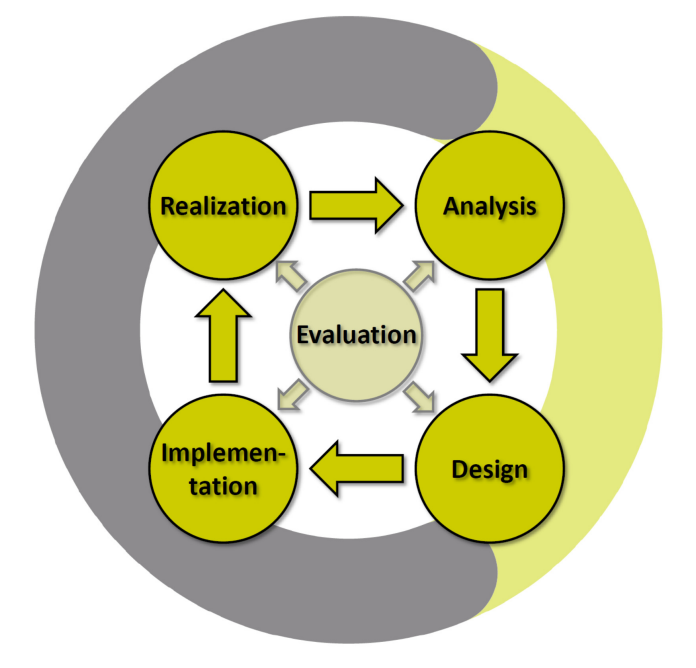
\includegraphics[width=0.75\linewidth]{fases.png}
    \caption{Fases del desarrollo del Marco de referencia de calidad para MOOCs}
    \label{fig:fases-calidad}
\end{figure}

\subsection{Perspectivas}
Las perspectivas se pueden entender como las características objetivo de cada uno de los procesos de las fases: pedagógicas, tecnológicas, estratégicas.

Esto se puede ver con un ejemplo, en la fase de implementación, en el proceso de implementación de contenido, existen dos perspectivas principales: tecnológicas y pedagógicas, ya que solo se engloban aquellas tareas de implementación de los contenidos académicos y de soporte de ese contenido.

\subsection{Roles}
En esta dimensión se encuentran a aquellos actores que tengan alguna responsabilidad o estén involucrados en los procesos de las fases.
\begin{enumerate}
    \item \textbf{Diseñador:} Se engloban los expertos en contenido, autores de contenido, diseñadores gráficos y expertos en plataformas LMS, así como todos los individuos que puedan contribuir al diseño del MOOC.
    \item \textbf{Facilitador:} Se engloban los expertos pedagógicos como tutores, moderadores y profesores, así como todos los individuos que puedan contribuir al proceso de aprendizaje del MOOC.
    \item \textbf{Proveedor:} Se engloban los proveedores técnicos como programadores, soporte técnico, desarrolladores de software así como todos los individuos que puedan contribuir a la toma de decisiones que lleven a la entrega del software del MOOC.
\end{enumerate}

\section{Buenas prácticas en la docencia en línea}
En la docencia en línea al igual que en el desarrollo software existen unas buenas prácticas que es conveniente seguir por el equipo educativo. Estas buenas prácticas se pueden ilustrar con experiencias de alumnos de UBUVirtual\cite{ubu-virtual}. Además de los conceptos encontrados en el libro Strategies for Effective Online Teaching and Learning: \cite{inbook}.

\subsection{Retroalimentaciones a tiempo}
El personal docente debe proporcionar retroalimentaciones a los estudiantes a tiempo, de esta forma se conseguirá que el alumno siga una cronología acorde a la del curso y pueda llevar una mejor organización de sus objetivos.
\subsection{Recursos actualizados}
Los recursos que el equipo docente ponga a disposición del alumnado, que pueden ser enlaces,libros,apuntes,vídeos,cuestionarios,simuladores y otros, deben estar actualizados. Para ello se deben hacer comprobaciones regularmente, de esta forma el alumnado tendrá todas las herramientas necesarias a su disposición sin incidencias. 
\subsection{Seguimiento del alumnado}
Un seguimiento continuo de la evolución del alumnado puede dar al equipo docente información clave para definir el avance del curso con el mayor éxito posible. Para realizar un buen seguimiento el docente se puede servir de cuestionarios, actividades, gráficas y otras herramientas que ofrecen los LMS.
\subsection{Priorizar la comunicación y las estrategias de interacción.}
El principal problema de la docencia en línea es la comunicación. En la docencia presencial, los alumnos ven diariamente a sus profesores y viceversa, esto facilita la comunicación y la capacidad del profesor para analizar el impacto en vivo que generan los contenidos impartidos en sus alumnos. 

Sin embargo, en la docencia en línea la información que el profesor puede obtener de las comunicaciones es más limitada, por lo que tiene que crear nuevas formas de comunicarse, que proporcionen la mayor cantidad de información posible para impartir una docencia de mayor calidad. 

Esto se tendrá que realizar mediante el uso de herramientas conocidas como foros,tablones de anuncios, grupos o correos. Pero estas herramientas tan usadas no proporcionan una línea de comunicación continua y duradera en un espacio temporal como lo puede hacer conversación presencial, por lo que una muy buena práctica sería proporcionar formas de conversar entre el equipo docente y el alumnado. Esto se puede hacer implementado chats, o haciendo llamadas por medios como Skype o Teams. Además se pueden hacer reuniones semanales para discutir con lo alumnos el avance del curso y los aspectos a mejorar por ambas partes.

\subsection{Evaluación objetiva mediante cuestionarios} 
Los cuestionarios son una herramienta muy útil para conocer el nivel de conocimientos de los estudiantes. Los cuestionarios nos ofrecen información sobre la actitud del alumnado hacia el curso, el nivel académico de los estudiantes, la evolución y otros datos. Además los LMS ofrecen esta funcionalidad de una forma muy completa, en el caso concreto de Moodle, existen distintas estadísticas que se pueden revisar.Esto se puede ver con ejemplos de la documentación oficial\cite{estadisticas-examen}. Estas estadísticas proporcionan al personal académico la capacidad de detectar preguntas que están mal planteadas, entender como responden los alumnos a las preguntas y asegurar que las variantes aleatorias no afecten en exceso a los resultados:

\begin{enumerate}
    \item \textbf{Índice de facilidad:} indica el porcentaje medio de la puntuación de los estudiantes en una pregunta, lo que se puede interpretar como dificultad de la pregunta. La tabla \ref{tabla:indice-facilidad} muestra los intervalos recomendados de los índices de facilidad y su interpretación.

    \tablaSmall{Porcentaje de índices de facilidad con sus dificultades}{l c}{indice-facilidad}
    { \multicolumn{1}{l}{Índice de facilidad} & Interpretación\\}{ 
    5\% o menos & Extremadamente difícil\\
    6\% - 10\%  & Muy difícil\\
    11\% - 20\% & Difícil\\
    21\% - 34\%  & Moderadamente difícil\\
    35\% - 65\% & Correcta para el estudiante promedio\\
    66\% - 80\%  & Bastante fácil\\
    81\% - 89\%  & Fácil\\
    90\% - 94\%  & Muy fácil\\
    95\% - 100\%  & Extremadamente fácil\\
    }

    Además, también se puede consultar la fórmula que se utiliza para obtener dicho índice:
    \begin{center}
        \begin{math}
            F_{i} = 100\frac{\bar{x_{i}} - x_{i}(min)}{x_{i}(max) - x_{i}(min)}
        \end{math}
    \end{center}
    
    \item \textbf{Calificación aleatoria estimada:} muestra el resultado medio de una pregunta con respuestas aleatorias, interesante para evitar el fraude, ya que si el porcentaje es 0\% significa que los alumnos nunca podrán aprobar el cuestionario respondiendo a las preguntas aleatoriamente.
    
    \item \textbf{Índice discriminatorio:} Este índice se basa en la idea de que si un alumno ha respondido bien al resto de preguntas del cuestionario, debe responder bien a la pregunta.
    \begin{center}
        \begin{math}
            D_{i} = 100r({x_{i},T}) = 100\frac{C(x_{i}, T)}{\sqrt{V(x_{i})V(T)}}
        \end{math}
    \end{center}
    
    \item \textbf{Índice de participación:} Este índice muestra la participación que están teniendo los cuestionarios de un curso comparando los estudiantes de un curso y la participación de un cuestionario.

    \item \textbf{Coeficiente de consistencia interna:} Este coeficiente se utiliza para diferenciar a los alumnos con mejor desarrollo o más  habilidosos del resto. Con este índice se puede saber si las preguntas de un examen son buenas discriminando entre estudiantes o si el cuestionario es homogeneo en cuanto a calidad. Un 75\% es considerado un valor correcto para este índice.
    \begin{center}
        \begin{math}
            CIC = 100\frac{P}{P-1}(1 - \frac{1}{V(T)}\sum_{p\in P} V(x_{p})) 
        \end{math}
    \end{center}    
\end{enumerate}

\section{Plan de calidad para cursos e-Learning}
Una vez vistos los conceptos básicos en los que se han basado los avances realizados en el proyecto, ahora se combinarán todos los conceptos explicados para obtener un plan de calidad sobre el que se basan las reglas implementadas de la aplicación. En este plan se combinan las distintas dimensiones del marco de referencia de calidad para MOOCs\cite{quality-reference-framework} junto con las buenas prácticas definidas. En la tabla \ref{tabla:2} se encuentran los objetivo de calidad que deseamos, la responsabilidad para los roles, las perspectivas de cada uno de los objetivos y el proceso del marco de calidad 
para MOOCs. 

\newpage

\begin{center}
    \rowcolors {2}{gray!35}{}
    \centering
    \label{tabla:2}
    \begin{longtable}{p{3cm} c c c c c}
            \caption{Consultas de calidad clasificadas en pespectivas y roles.\\
                Leyenda:\\
                \textbf{Responsabilidad:} R=Responsable X=Involucrado\\
                \textbf{Perspectivas:} P=Pedagógica T=Tecnológica E=Estratégica \\
                \textbf{*:} Nueva Regla
            }\\
        \hline
        Consulta & Perspectivas & Diseñador & Facilitador & Proveedor & Proceso\\
        \endhead
        \hline
        Las opciones de progreso del estudiante están activadas & P + T & R & X & & D-5 \\
        \hline
        Se proporcionan contenidos en diferentes formatos & P + T & R  & X & X & D-4\\
        \hline
        El curso tiene grupos & P & R & X & X & D-5 \\
        \hline
        El curso tiene actividades grupales & P & R & X & X & D-3 \\
        \hline
        Los estudiantes pueden ver las condiciones necesarias para completar una actividad & P & R & X & X & \\
        \hline
        Todas las actividades tienen la misma nota máxima en el calificador & P & R & X & X & \\
        \hline
        El curso tiene fechas y descripción definidas * & P + E & R & X & X & \\
        \hline
        Las preguntas de los cuestionarios tienen una calificación aleatoria adecuada * & P + T  & R & X &  & \\
        \hline        
        Las preguntas de los cuestionarios tienen retroalimentación & P & R & X &  & \\
        \hline
        Las preguntas de opción múltiple puntúan con una calificación aleatoria estimada de cero & P + T & R & X & X & \\
        \hline
        Los recursos están actualizados & P + T & R & X & X & I-1 \\
        \hline
        Fechas de apertura y cierre de tareas son correctas & P + T & X & R & X & R-2 \\
        \hline
        Se detallan los criterios de evaluación (rúbricas, ejemplos) & P + T & R & X & X & R-3 \\
        \hline
        El calificador no tiene demasiado anidamiento & P + E & R & X & X & \\
        \hline
        Los alumnos están divididos en grupos & T + E & X & & R & I-6 \\
        \hline
        El profesor responde en los foros dentro del límite de 48 horas lectivas desde que se plantea la duda & P + T + E & X & R & X & R-2 \\
        \hline
        Se ofrece retroalimentación de las tareas & P + T + E & X & R & X & R-2 \\
        \hline
        Las tareas están calificadas & P + T & X & R & X & R-2 \\
        \hline
        El calificador muestra cómo ponderan las diferentes tareas & P + T + E & X & R & X & R-2 \\
        \hline
        El tiempo de los cuestionarios está bien ajustado & P & R & X & X & \\
        \hline
        Los cuestionarios tienen una dificultad estimada entre unos valores umbrales & P + T + E & R & X & X & \\
        \hline
        Las preguntas de los cuestionarios son buenas discriminando & P + T + E & R & X & X & \\
        \hline
        Los índices de facilidad de las preguntas son adecuados * & P + T + E & X & R & X & R-2 \\
        \hline
        Los cuestionarios tienen una participación adecuada * & P + T + E & X & R & X & R-2 \\
        \hline     
        Las preguntas de los cuestionarios tienen un índice de discriminación adecuado * & P + T + E & X & R & X & R-2\\
        \hline     
        Los cuestionarios tienen un coeficiente de consistencia interna adecuado * & P + T + E & X & R & X & R-2\\
        \hline             
        La mayoría de alumnos responden a los feedbacks & P + T + E & X & X & R & E-2 \\
        \hline
        Se utilizan encuestas de opinión & P + T + E & X & X & R & E-2 \\
        \hline
    \end{longtable}
\end{center}

\capitulo{4}{Técnicas y herramientas}

Esta parte de la memoria tiene como objetivo presentar las técnicas metodológicas y las herramientas de desarrollo que se han utilizado para llevar a cabo el proyecto. Si se han estudiado diferentes alternativas de metodologías, herramientas, bibliotecas se puede hacer un resumen de los aspectos más destacados de cada alternativa, incluyendo comparativas entre las distintas opciones y una justificación de las elecciones realizadas. 
No se pretende que este apartado se convierta en un capítulo de un libro dedicado a cada una de las alternativas, sino comentar los aspectos más destacados de cada opción, con un repaso somero a los fundamentos esenciales y referencias bibliográficas para que el lector pueda ampliar su conocimiento sobre el tema.



\capitulo{5}{Aspectos relevantes del desarrollo del proyecto}

\section{Arreglar el fallo con las nuevas versiones de Moodle}
Al menos el 60\% de los costes de un software va dirigido al mantenimiento, ya sea correctivo o adaptativo a nuevas funcionalidades \cite{costos-mantenimiento}. Esta aplicación necesitaba mantenimiento y actualización. Generalmente en el mantenimiento del software nos encontramos con problemas constantemente y es deber de los ingenieros solucionarlos, además de documentar esos problemas y los pasos que se han realizado para solucionarlos, para que en el futuro si vuelven a fallar las mismas cosas, otros desarrolladores tengan una guía de como solucionar dicho error, facilitando el trabajo en el futuro. Un buen método para hacer esto es el conocido como proceso ACR (Análisis de causa raíz).\cite{proceso-acr}.

\subsection{Planteamiento del problema}
Al inicio de este proyecto la aplicación fallaba con las versiones de Moodle superiores a la 4.0 . La información que obtuvimos era poca, recibíamos un puntero a nulo en algún punto del código.
\subsection{Análisis y obtención de datos}
Para solucionar el problema, se ha estudiado los puntos en los que se generaban los errores, y se han obtenido datos de todas las trazas de los errores. Esto se ha conseguido gracias a un análisis de la aplicación minucioso con la función de debug del IDE.
Además, se ha probado la aplicación con la versione 3.9 de Moodle, en este caso la aplicación funcionaba correctamente.

Esto lleva a pensar que algún dato de la Web API de Moodle ha cambiado, generando un nulo al intentar mapear dicho dato en la aplicación.

Tras más pruebas pudimos detectar que este error se debía a la variable visible de algunas respuestas de la Web API de Moodle. Esta variable ha cambiado de tipo desde la versión 3.10 hasta las nuevas versiones, provocando fallos en el mapeo. Esto debido que la aplicación dispone de un modelo que representa los datos que se reciben desde la Web API de Moodle en formato JSON. Estos datos se guardan en atributos en las distintas clases del modelo. El cambio de tipo de entero a booleano en uno de los datos ha generado una incompatibilidad con varias clases del modelo. 

\subsection{Solución}
La solución elegida ha sido interceptar el dato antes de mapearlo en nuestra aplicación. Esto consiste en recibir los datos en formato JSON de la Web API de Moodle, localizar los tipos que generan conflicto y convertirlos manualmente al tipo que interesa, seguidamente se podrá vincular al atributo de la clase. De esta forma la aplicación funciona correctamente tanto para las versiones anteriores como las nuevas. Es una solución que se asemeja a un microservicio de interceptación \cite{interceptor}.

Esta interceptación se podía hacer de varias formas, nosotros hemos optado por hacerla en el mismo servicio, pero existen formas para hacerlo en la clase que hace la llamada a la API\cite{spring-interceptor}.

\section{Arreglar la portabilidad del proyecto con ejecutable .war}
Una de las ventajas de Spring Boot es la capacidad de crear y configurar aplicaciones portables rápidamente. Sin embargo la portabilidad de nuestra aplicación fallaba, por lo que no estábamos aprovechando esas ventajas que proporciona Spring Boot al máximo. 
\subsection{Planteamiento del problema}
El problema encontrado es que al ejecutar el comando: 
"java -jar prototipo-0.4-SNAPSHOT.war", el error que recibíamos era un puntero a nulo en varios lugares del código. Este error no permitía mostrar páginas más que las de manual de usuario. y ``about''. Como dato importante, el ejecutable si que funcionaba cuando estaba en el target que genera Maven al ejecutar el comando "mvn install".
\subsection{Análisis y obtención de datos}
Tras analizar el código hemos podido descubrir que los nulos proceden de todas las instrucciones que utilizaban alguna ruta predeterminada, por lo que podemos suponer que el problema se originaba de la obtención de ficheros mediante rutas. 

\subsection{Solución}
Para solucionar este problema hemos decidido aprovechar la carpeta de recursos que la extensión de Spring Boot empaqueta con nuestro .war \cite{read-file-from-resources}. De esta forma se asegura que todos los ficheros que utiliza el código estén dentro del .war y alcanzables en todo momento.

Por otro lado, hemos cambiado la forma de obtener los ficheros en el código utilizando los InputStream \cite{inputstream}.

\section{Implementación de Docker en el proyecto}
Una de las nuevas características de este proyecto es la capacidad de  ser desplegado con Docker \cite{docker}. Con Docker la aplicación puede ser desplegada con rapidez y eficiencia en numerosos entornos, además abre la posibilidad de dividir el frontend y el backend y ser igual de rápido y eficiente que ahora. Esto permitirá tener una interfaz mas completa e interesante de lo que pueden ofrecer las hojas JSP.

\section{Nueva regla: Definición de fechas y descripción del curso}
En el marco de calidad QRF \cite{quality-reference-framework} uno de los estándares de calidad es la correcta definición del curso en la fase de diseño, esto incluye especificar una fecha de inicio y una fecha de fin. Esto ha definido un requisito funcional para la aplicación.

Para la implementación de esta regla se utiliza la API que proporciona información general sobre cada curso. Entre esta información se encuentra la descripción del curso, que si se encuentra como un String vacío se interpreta que no tiene y las fechas que se devuelven en formato``timestamp'', que si es 0 significa que no están definidas. Con estos datos, se ha programado esta regla que permite a los profesores saber si están cumpliendo estas sencillas condiciones para tener un curso de calidad.

\section{Implementación de gestión de sesión para web scraping}
Una de las barreras para la implementación de muchas de las reglas que nos proporcionan los marcos teóricos es la falta de información, esto debido a que la API de Moodle \cite{moodle-api} no proporciona todos los datos necesarios para implementar ciertas reglas. Por ello es necesario la implementación de funcionalidades que se sirvan de web scraping para la obtención de esta información. Pero para obtener los datos mediante web scraping también surgen algunos problemas.

\subsection{Planteamiento del problema}
Se necesita obtener datos de la página de Moodle, ya que la API de Moodle no proporciona los datos necesarios. Para poder acceder a la página de Moodle se necesita una sesión de la que no se dispone mediante la API.

\subsection{Análisis y obtención de datos}
Siempre que se inicia sesión en Moodle desde su página se obtiene una sesión para poder acceder y realizar operaciones. Con esa sesión se podría obtener los datos necesarios desde la aplicación y de esa forma calcular las reglas

\subsection{Solución}
En base a una solución similar de UbuMonitor \cite{ubu-monitor}, se ha creado una clase que gestiona la sesión del usuario, para que este disponga de una llave de sesisón que podrá introducir en aquellas peticiones que se hagan desde la web y no de la Web API de Moodle. De esta forma se abren las puertas al web scraping y se multiplican las posibilidades de implementación de reglas. 

\section{Implementación de reglas de cuestionarios}
Una de las principales herramientas que permiten acreditar la comprensión de los contenido impartidos en un curso son los cuestionarios \cite{evaluacion-de-educacion-virtual}. Desde la perspectiva estratégica los cuestionarios guían a los involucrados en el proceso educativo mostrando la adaptación y el desarrollo de los estudiantes en el curso y sus contenido.

Dado que los cuestionarios son tan importantes, también es importante que estén bien hechos y con un mínimo de calidad para asegurar el máximo aprovechamiento de la herramienta. Por ello, se han definido reglas en este proyecto que permiten al usuario ver varios datos importantes para la calidad de cuestionarios.

En cuanto a la implementación de reglas de este tipo, esta aplicación utiliza datos que proporciona la Web API de Moodle \cite{moodle-api} e informes estadísticos \cite{estadisticas-examen} que tienen a su disposición los profesores y tutores con permisos en su organización. Para la obtención de los informes estadísticos se ha utilizado web scraping \cite{web-scraping}. Además, para todos las reglas, sin incluir la regla de calificación aleatoria se utilizan los  cuestionarios visibles y con fecha de finalización inferior a la fecha actual o sin fecha de finalización definida. 

\subsection{Nueva regla: Los cuestionario tiene una participación mínima}
La finalidad de los cuestionarios es que el facilitador pueda ver si sus alumnos están entendiendo los contenidos impartidos. Si los alumnos no realizan estos cuestionarios el facilitador no puede aprovechar esta herramienta. Por ende, para poder sacar conclusiones de los resultados de los cuestionarios es importante que un mínimo de alumnos participe en ellos. 

Con estas bases se ha diseñado e implementado una nueva regla en el proyecto. En esta nueva funcionalidad se compara los estudiantes de un curso con los participantes de un cuestionario finalizado. De esta comparación se obtiene un porcentaje y si está por debajo del valor definido en el fichero de configuración se considera que el cuestionario tiene una baja participación.

El porcentaje de participación en caso de que sea baja se muestra al usuario para que pueda tomar las medidas convenientes para aumentar esa cifra, los valores recomendables se encuentran por encima del 80\%.

\subsection{Nueva regla: Los cuestionarios tienen un índice de facilidad correcto}
El índice de facilidad es la puntuación media de los alumnos en una pregunta de un cuestionario.Esta estadística que proporciona Moodle en su reporte estadístico de cuestionarios ayuda a entender a los facilitadores y diseñadores la dificultad de los cuestionarios. Según la documentación de Moodle respecto a las estadísticas de cuestionarios \cite{estadisticas-examen} los valores adecuados para el estudiante medio se encuentran entre el 35\% y 65\%.

Para la implementación de esta regla, se lee del archivo de estadísticas de cuestionarios el índice de facilidad de cada pregunta y se realiza una media con todos los índices obtenidos para obtener un índice de facilidad global del cuestionario. Si el índice de facilidad del cuestionario está fuera del intervalo estipulado se considera que el cuestionario no está bien planteado. En caso de que el cuestionario este mal planteado se muestran las preguntas que tienen un índice de facilidad incorrecto. Para que el facilitador sepa donde tiene que hacer cambios para mejorar la calidad del cuestionario.

Esta regla da una guía clara a los facilitadores e incluso a los diseñadores para entender el nivel al que están los estudiantes y la posible necesidad de adaptar los recursos del curso a las necesidades de los estudiantes. 

\subsection{Nueva regla: Los cuestionarios tienen un índice de de calificación aleatoria adecuado}
El índice de calificación aleatoria es la media de calificación que el estudiante obtendría realizando la pregunta en cuestión aleatoriamente. Este índice solo esta disponible para preguntas de opción múltiple. El objetivo de esta estadística es que los profesores sepan cuál podría ser la calificación máxima de un estudiante sin que tenga conocimiento alguno sobre la pregunta. Según la documentación oficial de Moodle \cite{estadisticas-examen} los valores correctos se encuentran por debajo del 40\% en cada pregunta.

Para implementar esta regla se lee el índice del archivo de reporte estadístico de cada cuestionario y se realiza una media con todas las preguntas contadas y se obtiene un porcentaje. Si este porcentaje supera un valor definido se considera que está mal planteado, por lo que sería necesario corregir algunas preguntas para considerarse correcto.

\subsection{Nueva regla: Los cuestionarios tienen un índice de discriminación adecuado}
El índice de discriminación relaciona la puntuación en una pregunta con las puntuaciones del resto de las preguntas. Este índice indica la efectividad de la pregunta para diferenciar a los estudiantes más hábiles en la materia de los que no lo son. Según la documentación oficial \cite{estadisticas-examen} una buena discriminación se encuentra por encima del 50\%.

Para implementar esta regla se accede nuevamente al fichero de estadísticas de cuestionarios y se lee el índice de cada pregunta, con los índices de todas las preguntas se hace una media y se comprueba que esa media este por encima de un valor definido. Si esta por debajo se considera que el cuestionario esta mal planteado y requiere revisión. Con el fin de localizar las preguntas que requieren revisión, se muestran las preguntas con sus respectivos índices.

Con este índice los facilitadores podrán identificar aquellas preguntas de los cuestionarios que no se adaptan correctamente al nivel de los estudiantes.
\subsection{Nueva regla: Los cuestionarios tienen un coeficiente de consistencia interna adecuado}
El coeficiente de consistencia interna se utiliza para hacer una discriminación entre estudiantes de distinta habilidad. Los valores adecuados se encuentran por encima de un 75\%. Cuando el valor está por debajo del 60\% se considera que se deben tomar medidas correctivas, ya que es posible que los resultados estén asociados al azar o que las preguntas estén evaluando una calidad diferente que el resto de preguntas por lo que el cuestionario no es homogeneo en su conjunto.

A este coeficiente está vinculada la tasa de error que dado los valores de la siguiente tabla se puede determinar que porcentaje de los resultados se deben a efectos aleatorios y cuales a diferencias en la habilidad del estudiante.


\tablaSmall{Relación entre coeficiente de consistencia interna y tasa de error}{l c}{1}
{ \multicolumn{1}{l}{Coeficiente de consistencia interna} & Tasa de error\\}{ 
100 & 0\\
99  & 10\\
96 & 20\\
91  & 30\\
84 & 40\\
75  & 50\\
64  & 60\\
51  & 70\\
} 

Los valores de la tasa indican el porcentaje de resultados dados por efectos aleatorios, siendo el restante el porcentaje de discriminación. Valores por encima del 50\% se consideran insatisfactorios.

\subsection{Diferencias entre versiones inferiores y superiores a 4.0 de Moodle}
Como se ha mencionado anteriormente, para la implementación de la mayoría de los cuestionarios ha sido necesaria la lectura de un fichero de reporte estadístico mediante web scraping. 

Sin embargo, uno de los problemas encontrado a la hora de implementar las funcionalidades ha sido que existen dos formatos para el fichero estadístico mencionado. En las versiones inferiores a la 4.0 de Moodle el fichero JSON está compuesto por arrays, sin claves que identifiquen que índica cada valor. A partir de la versión 4.0 el JSON tiene una mejor estructura con claves que identifican cada dato que se muestra.

Para la resolución de este conflicto ha sido necesario realizar una proceso intermedio en el que se identifica la versión del Moodle con el que se está trabajando, este dato se ha obtenido con la API de Moodle\cite{moodle-api}. Conociendo la versión se realiza la operación de obtención de índices de una forma u otra.

Con esto se logra que los usuarios de cualquier versión puedan acceder a las funcionalidades implementadas, de esta forma se obtiene un mayor alcance de usuarios.

\section{Implementación de funcionalidad de exportación de informe en Excel}
Hasta el momento, en la aplicación, para visualizar un informe ha sido necesario conectarse, generar un informe y visualizarlo en el momento. No existía la capacidad de guardar el informe de ningún modo, lo que suponía una dificultad para el usuario hacer un seguimiento completo en el tiempo. 

Para poder dar la opción de llevar un seguimiento de todos los informes de calidad generados existen dos opciones: que los informes de calidad sean mostrados por la aplicación o que el usuario pueda tener uno o varios archivos con los informes de calidad que desee. Para la primera opción sería necesario guardar los informes en una base de datos o en una carpeta con los informes de calidad guardados en archivos tipo JSON, Excel o incluso imagen. Sin embargo, esta opción aumentaría mucho la complejidad, por lo que resulta más atractiva la segunda opción.

En virtud de lo cual, se optó por implementar la funcionalidad de exportación de informes de calidad a Excel formato ".xlsx". Para esta implementación, se ha diseñado una plantilla con las reglas y sus descripciones. A continuación, se ha implementado una función que rellena dicha plantilla con los datos del informe del curso en cuestión. Hay que puntualizar que solo se genera un Excel para cada curso, es decir, no se puede generar un Excel con los informes de calidad de varios cursos. Esta función es llamada desde la gateway que se utiliza desde la vista para obtener el Excel completo. 








\capitulo{6}{Trabajos relacionados}

Este apartado sería parecido a un estado del arte de una tesis o tesina. En un trabajo final grado no parece obligada su presencia, aunque se puede dejar a juicio del tutor el incluir un pequeño resumen comentado de los trabajos y proyectos ya realizados en el campo del proyecto en curso. 

\capitulo{7}{Conclusiones y Líneas de trabajo futuras}

Todo proyecto debe incluir las conclusiones que se derivan de su desarrollo. Éstas pueden ser de diferente índole, dependiendo de la tipología del proyecto, pero normalmente van a estar presentes un conjunto de conclusiones relacionadas con los resultados del proyecto y un conjunto de conclusiones técnicas. 
Además, resulta muy útil realizar un informe crítico indicando cómo se puede mejorar el proyecto, o cómo se puede continuar trabajando en la línea del proyecto realizado.


\bibliographystyle{plain}
\bibliography{bibliografia}

\end{document}
